\subsubsection{extractfeatures}

{\ttfamily extractfeatures} gets various data from an image in a collection
and saves it to feature files.
It uses a SIFT feature detector to determine keypoints in an image, which are 
later used to compare the image with other images in the collection. Details
for the SIFT method can be found in~\cite{lowe}.

\begin{verbatim}
USAGE: 

extractfeatures  [--bow <filename>] [--precluster <int>] [--clahe <int>]
                 [--sdk <int>] [--numbins <int>] [-o <string>] ...  [-n
                 <string>] ...  [-l <int>] [-v] [-d <string>] [--]
                 [--version] [-h] <file>


Where: 

   --bow <filename>
     [BOWHistogram] Bag of Words file

   --precluster <int>
     [SIFTComparison] Number of descriptors to select in preclustering 
	 (0 = no preclustering)

   --clahe <int>
     [SIFTComparison] Value of adaptive contrast enhancement 
	 (1 = no enhancement)

   --sdk <int>
     [SIFTComparison] Number of Spatial Distinctive Keypoints 
	 (0 = no SDK)

   --numbins <int>
     [ImageHistogram] Number of histogram bins

   -o <string>,  --only <string>  (accepted multiple times)
     extract only specified features

   -n <string>,  --no <string>  (accepted multiple times)
     exclude feature from extraction

   -l <int>,  --level <int>
     Characterization Level (1-3)

   -v,  --verbose
     Provide additional debugging output

   -d <string>,  --dir <string>
     Output directory for feature files.

   --,  --ignore_rest
     Ignores the rest of the labeled arguments following this flag.

   --version
     Displays version information and exits.

   -h,  --help
     Displays usage information and exits.

   <file>
     (required)  image file to extract features from
\end{verbatim}

\paragraph{CLAHE}


\begin{figure}
	\centering
		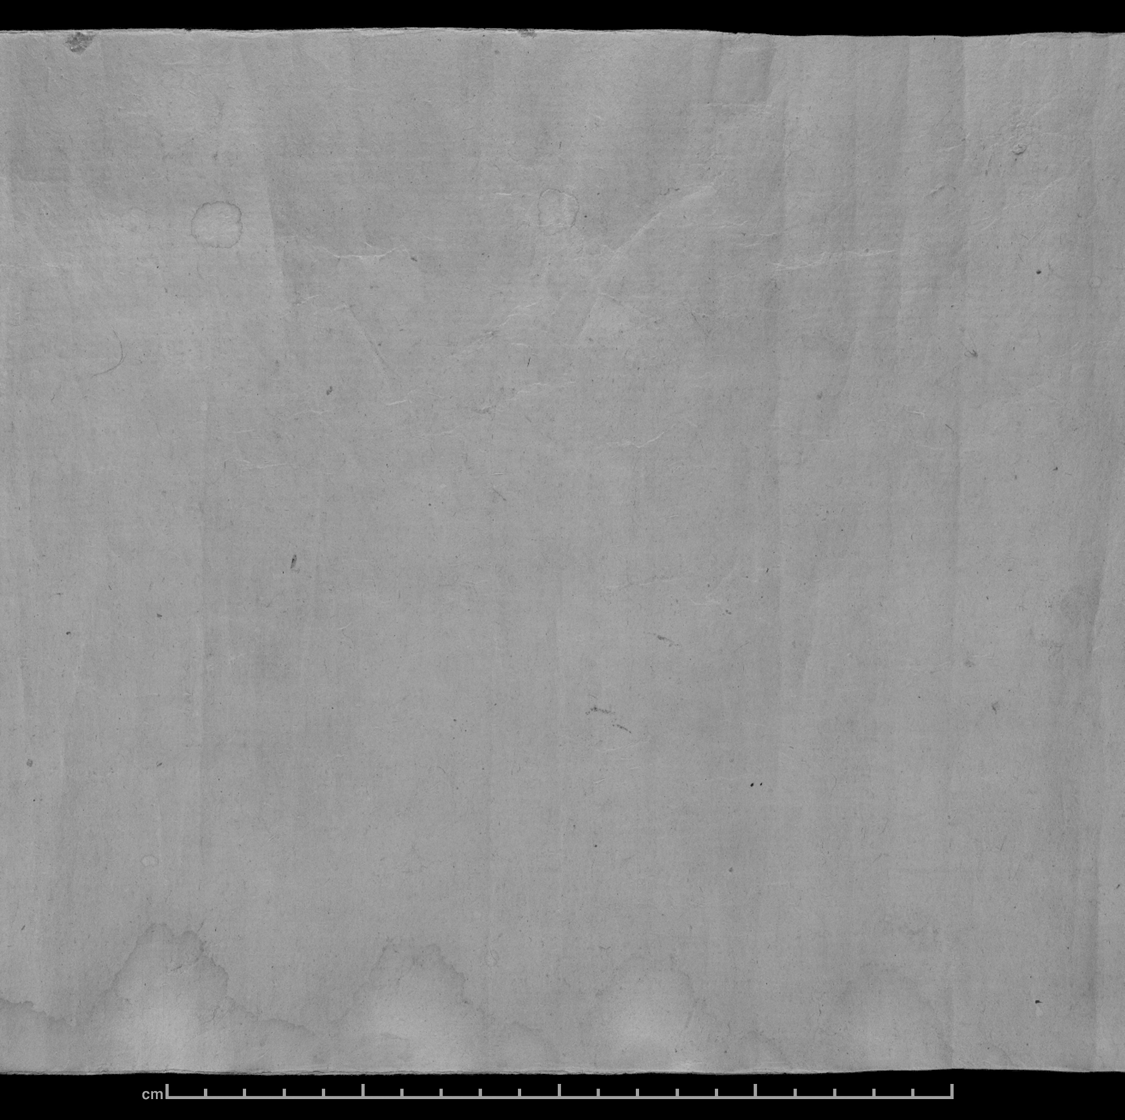
\includegraphics[width=0.80\textwidth]{img/BLX2565_OR8210S30VB_4_L_original.png}
	\caption{Original image without contrast enhancement}
	\label{fig:BLX2565_OR8210S30VB_4_L_original}
\end{figure}


\begin{figure}
	\centering
		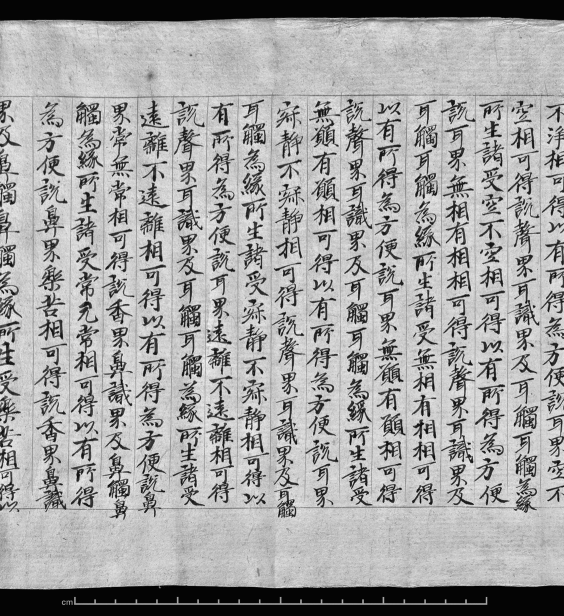
\includegraphics[width=0.80\textwidth]{img/BLX2605_OR8210S61R1_8_L_clahe.png}
	\caption{Image with contrast enhanecement}
	\label{fig:BLX2605_OR8210S61R1_8_L_clahe}
\end{figure}
